\subsubsection{Greedy--Algorithmus}
Wie schon im \cref{sec:definitionen} erwähnt wurde, können die Gedanken bezüglich des
\fp{} auf andere Größen übetragen werden. Da die Größen des Rechtecks $R$ sowie des Zeitraums fest sind
und auf 1000 Metern bzw. auf den Zeitraum von 8:00 is 18:00 beschränkt sind, konvertieren wir
die Eingabe, indem wir den Beginn des Zeitraumes auf 0 setzen, d.h., wir subtrahieren den 
Anfang $B$ vom Ende $E$. So bleibt auch der WErt $M$, also die Differenz von $E$ und $B$, gleich. 
Analog müssen wir Eingabe der kleineren Rechtecke $r_i$ entsprechend konvertieren, indem wir
von jedem $b_i$ und $e_i$ den Wert $B$ abziehen. Für"die Aufgabe hat diese Konversion keine
Bedeutung und funktioniert auch, wenn ein angegebener Zeitraum sich vom ursprünglichen Zeitraum unterscheidet.
Mit dieser Konversion können wir ebenfalls mehrtägige Flohmärkte oder
sogar mehrere unterschiedlichen Flohmärkte behandeln.
Wenn der angegebene Zeitraum an einer Stelle unterbrochen ist,
etwa von 7:00 bis 9:00 und dann von 12:00 bis 15:00, ist es auch kein Problem, dann kann der
Zeitraum von 7:00 bis 15:00 angegeben werden und die Zeiten zwischen 9:00 und 12:00 bleiben unbesetzt.
Mehrtägige Flohmärkte können auf dieselbe Weise behandelt werden: Die gesamte Öffnungszeiten des Flohmarktes können in Stunden angegeben werden, zum Beispiel der Zeitraum eines Flohmarkts, der zwei Tage von 10:00 bis 17:00 dauert, kann als von 10:00 bis 41:00 (17:00 + 24 Stunden) dargestellt werden. Mehrere unterschiedlichen Flohmärkte kann man analog kodieren. Es hängt nur von der Eingabe ab.
\TODO{Beipiele dazu}
\TODO{Erwähne Zeiten in Minuten}
Nach der Konversion der Eingabe bilden wir eine Liste $Z$, in der jedes
Rechteck $r_i$ mit seinen genannten Größen $s_i, b_i, e_i$ gespeichert.

Die Größen $N$ und $M$ sind im Programm fest, unabhängig davon, wie viel sie betragen.
Außerdem wurde im \cref{sec:definitionen} festegestellt, dass die Größen $s_i$, $b_i$ und $e_i$
des jeweiligen Rechtecks $r_i$ fest sind und dass wir nur ein Rechteck $r_i$ entlang der $x$--Achse,
also entlang der Seite der Länge $N$ des Rechtecks $R$ bewegen dürfen.
So bietet sich eine Verteilung der kleinere Rechtecke $r_i$ auf kleinere \textit{\textbf{Streifen}}
der Länge $N$ im Rechteck $R$ entlang der Seite der Länge $N$.
Die Breite eines solchen Streifen ist äquidistant für alle Streifen und, da
man Stände am Flohmarkt nur zu vollständigen Stunden vermieten kann, lässt sich
die Breite eines Streifens zu einer vollständiger Stunde bstimmen.
\TODO{Minuten erwähnen}
Im Programm sind diese Streifen einfach Listen mit allen kleineren Rechtecken, 
deren Breite $m_i$ sich in diesem Streifen enthält.
Legen wir die folgende Schreibweise fest: Ein Streifen im Rechteck $R$, der die
Stunde $k$ betrifft, also in der Stunde $k$ beginnt und in der Stunde $k+1$ endet, nennen wir $S_k$.
Das bedeutet, dass ein Rechteck von $b_i = 1$ (nach Konversion, in vollständigen Stunden)
und $e_i = 5$ in den folgenden Streifen enthalten wird: $S_1, S_2, S_3, S_4$. Im Streifen $S_5$
wird er nicht enthalten, da die Miete mit dem Anfang der 5. Stunde endet.
Wie Streifen implementiert werden, lesen Sie in der \nameref{sec:umsetzung}.

Nach dieser Vorbereitung der Eingabe erfolgt der Lauf unseres Greedy--Algorithmus, der das
Ausgangsergebnis liefert.
Wir sortieren die Rechtecke in jeder Liste $S_i$ unabhängig voneinander nach folgenden Kriterien
in dieser Reihenfolge: 
1) fallend nach dem Wert $e_i$,
2) aufsteigend nach dem Wert $b_i$ und
3) fallend nach der Fläche jedes Rechtecks. 
Somit sind die ersten Rechtecke in jeder Liste $S_i$ diejenigen,
deren Wert $e_i$ am größten ist --- oft diejenigen, die am breitesten im Streifen sind.
\TODO{warum diese Reihenfolge? najpierw załatwaimy od lewej największe, po prawej upychamy najmniejszymi}
Diese Reihenfolge wurde so gewählt, dass wir in dieser Reihefolge versuchen,
die Rechtecke aus den Streifen ins große Rechteck $R$ zu platzieren.

Stellen wir uns vor, die das Rechteck $R$ liegt auf auf einem Koordinatensystem.
Die Seite der Länge $N$ verläuft entlang der $x$--Achse und die Seite der Länge
$M$ entlang der $y$--Achse.
Der Wert $B$ (nach der Konversion) wird entsprechend am Punkt $(0, 0)$ abgebildet.
Wir verarbeiten Streifen für Streifen in der
aufsteigenden Reihenfolge der $y$--Werte beginned mit dem 0--ten Streifen.
Wir iterieren durch jede Liste $S_i$ und untersuchen jedes Rechteck $r_j$ in diesem
Streifen, ob sein Wert $b_j$ gleich dem Wert $i$, also ob das Rechteck (die Anmeldung) mit dem
aktuellen Zeitpunkt $i$ beginnt. Außerdem prüfen wir, ob ein Rechteck bereits platziert wurde.
Wenn ein 



Damit kann man sich vorstellen, dass wir das Rechteck $R$ quasi vom Punkt $(0,0)$ bis zum Punkt
$(N, E)$ mit kleineren Rechtecken füllen. Nach 

\begin{figure}[h]
\centering
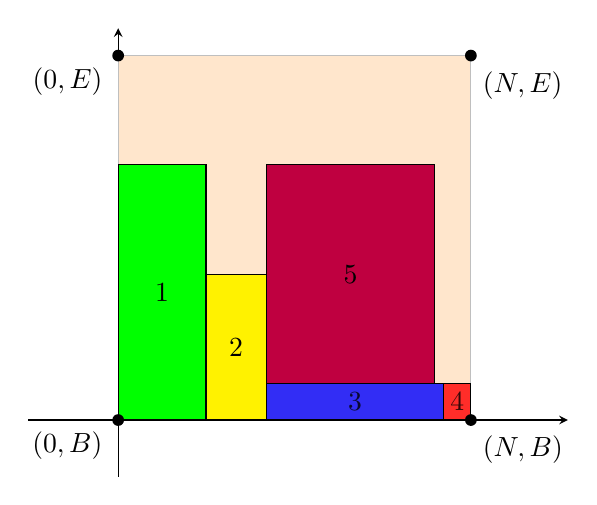
\begin{tikzpicture} 
\begin{axis}[
		ticks=none,
        xmin =-2.55,
        xmax = 12.75,
        ymax = 10.75,
        ymin = -1.55,
        axis x line = middle, axis y line = middle,
        every axis plot/.append style={ultra thick}]

	\draw [draw=lightgray, fill=orange, fill opacity=0.2] (0,0) rectangle (10, 10);
	\draw [fill = green] (0,0) rectangle node {1} (2.49, 7) ;
	\draw [fill = yellow] (2.49, 0) rectangle node {2} (4.2, 4) ;
	\draw [fill = blue, fill opacity = 0.8] (4.2, 0) rectangle node {3} (9.23, 1) ;
	\draw [fill = red, fill opacity = 0.8] (9.23, 0) rectangle node {4} (10, 1) ;
	\draw [fill = purple] (4.2, 1) rectangle node {5} (8.97, 7) ;
	\node[label={200:{$(0, B)$}},circle,fill,inner sep=1.5pt] at (axis cs:0,0) {};
	\node[label={290:{$(N, B)$}},circle,fill,inner sep=1.5pt] at (axis cs:10,0) {};
	\node[label={200:{$(0, E)$}},circle,fill,inner sep=1.5pt] at (axis cs:0,10) {};
	\node[label={290:{$(N, E)$}},circle,fill,inner sep=1.5pt] at (axis cs:10,10) {};
	%\draw [fill = yellow] (0,7) rectangle node {} (5.26, 10) ;
\end{axis} 
\end{tikzpicture}
\end{figure}




\TODO{wie werden die Rechtecke gelegt?\\
-- binary search\\
-- was sind die Folgen? was will man damit erreichen?}


